\chapter{Evaluation}
\label{Evaluation}

Closely following \Cref{Methodology}, the following chapter shows the extent and results of the performed tests.
It starts with the functional tests checking for correctness, continues with the accessibility evaluation, and ends with the comparative usability study.

\section{Functional Testing}
\label{Evaluation-Tests}

This section is divided into two parts reflecting significant differences in the types of tests used: low-level unit tests and high-level \gls{ui} tests.
Both sections outline the implementation, scope, and achieved results.

\subsection{Unit Tests}
\label{sec:evaluation-unit-tests}

To cover all important reusable parts (units) of the software, all files within the $/src/lib$ directory\footnote{Available at \href{https://github.com/durasj/chipsandcode/tree/4576a0b/src/lib}{github.com/durasj/chipsandcode/tree/4576a0b/src/lib}.} had a corresponding $.test.ext$ file.
The only exceptions were: Svelte components that would be better suited for Cypress Component Testing\footnote{Available at \url{https://docs.cypress.io/guides/component-testing/overview}.} --- which did not yet have stable support for Svelte, type definition files, and files that were tested indirectly.

Figure~\ref{fig:test-unit-example} shows an example unit test that belongs to the test suite for output processing.
It checks the output object can be created from text input, allows observing the loaded values, and can be serialized back.

In total, 181 unit tests spread over 16 test suites covered over 95\% of the 1500 targeted lines as can be seen in Figure~\ref{fig:test-coverage}.

Notably, excluded from this report is the coverage of all \gls{hdl} and \gls{tst} files making up the built-in and Project 1 chips from Nand2Tetris.
The built parsers were tested by using all (dozens) built-in and Project 1 files on the input with the expectation the output matches snapshots.
For example, for \gls{hdl}, these can be seen in the directory $/src/lib/editor/hdl/testing$.
The same applies to the introduced \gls{tst} parser.

Moreover, all produced \gls{ast} files were used to test the chip factory to verify it can process them.
This input was the same output parser tests produced, to prevent duplication.
One important limitation of this approach is these chip factory tests are no longer isolated as they require to be run after the parser tests.
However, in practice, after the first run, parser snapshots are persisted and do not change, which makes it, at most, a possible source of frustration for the developer adding new relevant tests.

\begin{figure}[H]
\centering
\begin{minted}[breaklines=true, fontsize=\small]{ts}
it('Can be created from existing output text', () => {
  const output = Output.fromText(`|   a   |   b   |  out  |
  |   0   |   0   |   1   |
  |   1   |   0   |   1   |`);

  expect(output.getRow(0)).toStrictEqual(
    [false, false, true]
  );
  expect(output.getRow(1)).toStrictEqual(
    [true, false, true]
  );

  expect(output.getText()).toBe(`| a | b |out|
| 0 | 0 | 1 |
| 1 | 0 | 1 |`);
});
\end{minted}
    \caption{Example unit test.}
    \label{fig:test-unit-example}
\end{figure}

\begin{figure}[H]
    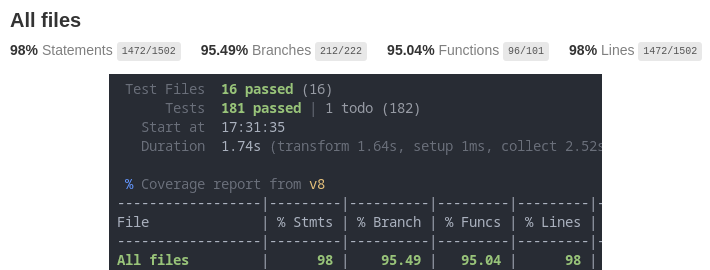
\includegraphics[width=380pt, keepaspectratio]{Unit_Coverage}
    \caption{Testing framework run output and coverage report.}
    \label{fig:test-coverage}
\end{figure}

\subsection{UI and Accessibility Tests}

Following the chosen methodology, the first step to writing \gls{ui} and accessibility tests was to identify all important use cases:

\begin{enumerate}
    \item User visits the home page, reads the welcome text, and uses the call-to-action button.
    \item User navigates to the learning content using the main menu.
    \item User navigates to the next section of the learning content using the side menu.
    \item User reads the learning content and navigates to the subsequent section using the "next" button.
    \item User navigates to the previous section using the "previous" button.
    \item User switches from the light theme to the dark theme while looking at the learning content.
    \item User interacts with the embedded Hardware \gls{ide}.
    \item User navigates to the Hardware \gls{ide} using the main menu.
    \item User loads the example Xor chip in the Hardware \gls{ide}.
    \item User changes the input for the Xor chip in the Hardware \gls{ide} and observes the result.
    \item User changes the Xor chip's definition in the Hardware \gls{ide} and observes the result.
    \item User changes the Xor chip's test script in the Hardware \gls{ide} and observes the results.
    \item User changes the Xor chip's expected output in the Hardware \gls{ide} and observes the results.
    \item User switches from the light theme to the dark theme while at the example Xor chip.
    \item User creates a new Experiment.
    \item User changes an Experiment name.
    \item User copies the link to the Experiment using the share functionality.
    \item User downloads and deletes an Experiment.
    \item User opens the About page using the main menu, reads the content, and opens links.
    \item User opens the sign-in page and reads the text.
\end{enumerate}

These use cases were grouped by the screen they were related to and implemented as Cypress tests.
As part of the test, all pages are checked for accessibility violations\footnote{Using aXe, see \url{https://github.com/dequelabs/axe-core/blob/0316e72/doc/rule-descriptions.md} for the list of performed checks.}.
Additionally, the same pages were also checked for visual regressions using a plugin\footnote{A Cypress plugin, available at: \url{https://github.com/FRSOURCE/cypress-plugin-visual-regression-diff}.} that calculated the difference between the captured and persisted screenshots.
Importantly, all tests are completely isolated, and all \gls{api} calls were stubbed to ensure there are no side effects.
Cypress automatically clears any state produced within the browser, but any state other side effects would create would not be cleared.

Figure~\ref{fig:test-cypress-example} shows an example Cypress test that belongs to the test suite for the home page.
It opens the page, checks it contains the heading, performs visual regression tests and accessibility checks, and verifies the call-to-action button redirects correctly.

Altogether, the software passed 19 tests spread over five test suites as can be seen in Figure~\ref{fig:test-cypress}.

\begin{figure}[H]
\begin{minted}[breaklines=true, fontsize=\small]{ts}
describe('Home', () => {
  it('Contains welcome message and link to content', () => {
    cy.visit('/');
    cy.injectAxe();

    cy.contains('Wondering how computers work?');

    cy.matchImage();

    cy.checkA11y();

    cy.contains('Start Learning').click();

    cy.location('pathname').should('eq', '/learn/hardware/boolean-logic');
  });
});
\end{minted}
    \caption{Example simplified Cypress test.}
    \label{fig:test-cypress-example}
\end{figure}

\begin{figure}[H]
    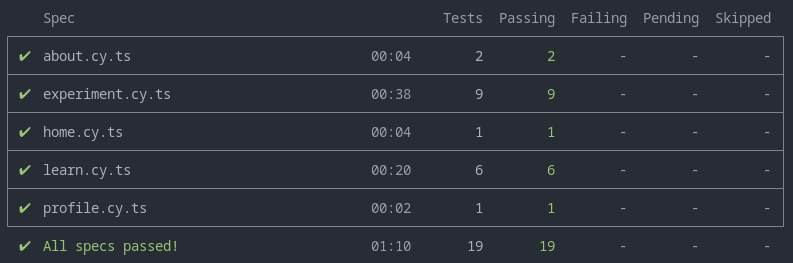
\includegraphics[width=380pt, keepaspectratio]{Cypress_Output}
    \caption{Output from Cypress run.}
    \label{fig:test-cypress}
\end{figure}

As mentioned in the methodology, not all use cases were covered.
These consisted of the following known use cases:

\begin{enumerate}
    \item \textbf{Chip Download}: This functionality was not covered as it is not trivial to test downloads in Cypress, especially if we consider it is a zip file that would have to be opened and inspected.
    \item \textbf{Dark Mode}: While this functionality is covered using visual regression tests to some extent, since it can be activated anywhere, it would require testing the same functionality in both modes everywhere. As this functionality is considered a "nice to have" opt-in feature, it was not considered worth it.
    \item \textbf{Responsivity}: Similarly to the previous point, the application can be used in all kinds of environments with a basically unlimited range of screen sizes. While testing the same functionality on a large range of screen sizes could be valuable, it was not possible with the limited time allocated to the thesis.
\end{enumerate}

\section{Accessibility Evaluation}
\label{Evaluation-Accessibility}

First of all, accessibility of the website was tested using aXe core\footnote{Available at \url{https://github.com/dequelabs/axe-core}.} during the Cypress test run.
In total, seven invocations to test accessibility of various pages in several states were performed, and all passed.
There were three exceptions where accessibility checks had to be disabled:

\begin{itemize}
    \item \textbf{Empty Table Header} rule, which was confused by the use of MathML in table headers.
    \item \textbf{Landmark Unique} rule, which was getting triggered on Monaco editor that is independent.
    \item \textbf{Colour Contrast} rule, which was triggered on Monaco Editor, but the editor provides an opt-in high contrast mode.
\end{itemize}

Secondly, an automated evaluation using browser extensions --- Lighthouse\footnote{Available at \url{https://chrome.google.com/webstore/detail/lighthouse/blipmdconlkpinefehnmjammfjpmpbjk}.} and aXe DevTools\footnote{Available at \url{https://chrome.google.com/webstore/detail/axe-devtools-web-accessib/lhdoppojpmngadmnindnejefpokejbdd}.} built into the Chrome DevTools --- was performed.
Both tools reported no problems with accessibility, as can be seen in Figure~\ref{fig:lighthouse-report} and Figure~\ref{fig:axe-report}.

\begin{figure}[H]
    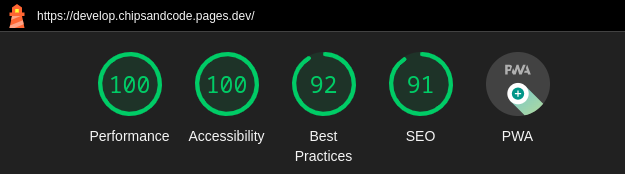
\includegraphics[width=380pt, keepaspectratio]{Lighthouse_Report}
    \caption{Lighthouse report summary.}
    \label{fig:lighthouse-report}
\end{figure}

\begin{figure}[H]
    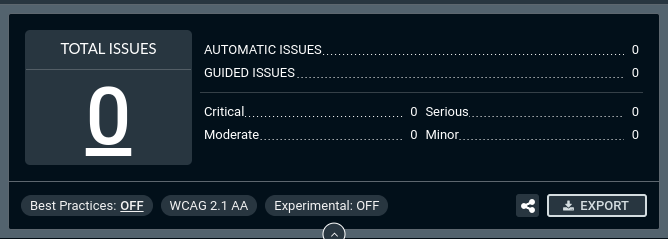
\includegraphics[width=380pt, keepaspectratio]{Axe_Report}
    \caption{aXe report summary.}
    \label{fig:axe-report}
\end{figure}

Lastly, a manual \gls{wcag} test, following the \gls{wcagem} report tool, was performed\footnote{Report can be found at \url{https://github.com/durasj/master-thesis/blob/main/assets/WCAG_Evaluation_Report.pdf}}.
The only potential problem identified during the testing involves dynamic updates to the \gls{ui}.
The author was unable to determine whether the automatically updated pin \gls{ui} is usable when using assistive technology.
For example, if the user changes some code in the editor and the list of pin updates, is this properly communicated using assistive technology?
Similarly, if the input on the pins changes, is it clear the output pin value is updated automatically, and can the user navigate to it easily?

Importantly, the software was not tested by third-party users who are either disabled or experienced in using assistive technologies.
While the author made the best effort to take into consideration accessibility, it is possible some of the checks were misunderstood.

\section{Comparative Usability Testing}
\label{Evaluation-UX}

The following section contains results from the comparative study.
All figures are also available at \href{https://thesis.chipsandcode.com}{thesis.chipsandcode.com} with the advantage of being interactive.

The total number of participants who joined the scheduled comparative study session was $n=26$.
Out of that, the data of two participants had to be removed --- Participant $F$, who experienced technical difficulties unrelated to the software and Participant $J$, who mentioned they tried the Proposed Software in the past.
The resulting sample size that was analysed was $n=24$, with an equal distribution of $n_1=12$ and $n_2=12$ among both groups.

The list of participants and their profiles within Group A can be seen in Table~\ref{table:evaluation-profile-a}, while Group B participant profiles can be seen in Table~\ref{table:evaluation-profile-b}.

\begin{table}[H]
    \centering
    \caption{Group A participant profiles.}
    \label{table:evaluation-profile-a}
    \begin{tabular}{ l l l l l l l l }
        \rotheading{Person} & \rotheading{Prior Exp.} & \rotheading{Education} & \rotheading{Occupation} & \rotheading{Age Group} & \rotheading{Paid} & \rotheading{Intr. Motiv.} & \rotatebox{30}{\textbf{Platform}} \\ \hline
        \textbf{M} & 1 & 2 & 2 & 30--49 & 0 & 0 & Ubuntu Linux desktop \\ \hline
        \textbf{LU} & 0 & 0 & 0 & 18--29 & 1 & 1 & Windows 10 laptop \\ \hline
        \textbf{Y} & 1 & 0 & 0 & 30--49 & 0 & 2 & Windows 10 laptop \\ \hline
        \textbf{MI} & 0 & 1 & 0 & 30--49 & 0 & 0 & Ubuntu Linux laptop \\ \hline
        \textbf{MX} & 1 & 2 & 1 & 30--49 & 0 & 1 & Windows 10 desktop \\ \hline
        \textbf{R} & 0 & 2 & 0 & 18--29 & 1 & 0 & Windows 10 desktop \\ \hline
        \textbf{MK} & 0 & 1 & 2 & 30--49 & 0 & 1 & Windows 11 laptop \\ \hline
        \textbf{L} & 0 & 2 & 2 & 18--29 & 0 & 1 & macOS 13 arm64 laptop \\ \hline
        \textbf{MA} & 0 & 0 & 0 & 18--29 & 1 & 1 & Windows 10 laptop \\ \hline
        \textbf{KY} & 0 & 1 & 1 & 18--29 & 1 & 1 & Windows 10 laptop \\ \hline
        \textbf{KA} & 0 & 0 & 0 & 18--29 & 1 & 0 & Windows 7 laptop \\ \hline
        \textbf{E} & 0 & 0 & 2 & 30--49 & 1 & 2 & Windows 10 desktop \\ \hline
    \end{tabular}
\end{table}

\begin{table}[H]
    \centering
    \caption{Group B participant profiles.}
    \label{table:evaluation-profile-b}
    \begin{tabular}{ l l l l l l l l}
        \rotheading{Person} & \rotheading{Prior Exp.} & \rotheading{Education} & \rotheading{Occupation} & \rotheading{Age Group} & \rotheading{Paid} & \rotheading{Intr. Motiv.} & \rotatebox{30}{\textbf{Platform}} \\ \hline
        \textbf{P} & 0 & 1 & 1 & 18--29 & 0 & 2 & Windows 10 laptop \\ \hline
        \textbf{S} & 0 & 1 & 0 & 30--49 & 0 & 1 & Windows 10 desktop \\ \hline
        \textbf{MM} & 1 & 1 & 2 & 18--29 & 0 & 1 & Ubuntu Linux laptop \\ \hline
        \textbf{SA} & 0 & 1 & 2 & 18--29 & 0 & 0 & Windows 11 laptop \\ \hline
        \textbf{JO} & 0 & 0 & 0 & 18--29 & 1 & 0 & Windows 11 desktop \\ \hline
        \textbf{PE} & 0 & 1 & 0 & 18--29 & 1 & 1 & Windows 11 laptop \\ \hline
        \textbf{MS} & 0 & 2 & 2 & 18--29 & 0 & 1 & Windows 11 laptop \\ \hline
        \textbf{B} & 1 & 2 & 2 & 18--29 & 0 & 1 & macOS 13 arm64 laptop \\ \hline
        \textbf{V} & 0 & 2 & 2 & 18--29 & 1 & 1 & Windows 10 laptop \\ \hline
        \textbf{MH} & 1 & 2 & 2 & 30--49 & 1 & 1 & macOS 13 x86 laptop \\ \hline
        \textbf{LB} & 0 & 2 & 2 & 18--29 & 1 & 1 & Windows 10 laptop \\ \hline
        \textbf{MT} & 0 & 2 & 0 & 18--29 & 1 & 2 & Windows 10 desktop \\ \hline
    \end{tabular}
\end{table}

As we can see, despite the effort to distribute participant profiles equally, the profiles were not completely equal between the groups.
To better capture the differences, Figure~\ref{fig:plot-points} shows the cumulative "Prior Experience", "Education", "Relevant Occupation", and "Intrinsic Motivation" between the two groups.
Additionally, Figure~\ref{fig:plot-age} shows the age make-up of the groups and Figure~\ref{fig:plot-platform} shows the platforms used by participants of each group.

\begin{figure}[H]
    \includesvg[width=380pt, keepaspectratio]{Plot_Points}
    \caption{Cumulative profile points between groups.}
    \label{fig:plot-points}
\end{figure}

\begin{figure}[H]
    \includesvg[width=380pt, keepaspectratio]{Plot_Age}
    \caption{Age characteristics of participants.}
    \label{fig:plot-age}
\end{figure}

\begin{figure}[H]
    \includesvg[width=380pt, keepaspectratio]{Plot_Platform}
    \caption{Platforms used by participants.}
    \label{fig:plot-platform}
\end{figure}

\subsection{Efficiency}
\label{sec:evaluation-efficiency}

The first kind of collected data on efficiency consisted of time-related data like the time it took to prepare the tool for use and time spent on individual tasks.
Figure~\ref{fig:plot-linear} shows a linear graph covering the mean of the time of mentioned steps between both groups.
The same data can be seen as cumulative, which is represented by Figure~\ref{fig:plot-stacked-bar}.
The total time spent on all parts was $512.42 \pm 190.01 s$ for Group A and $1,496.67 \pm 326.18 s$ for Group B ($\alpha=0.05$, $p<0.001$).
Raw data collected during the study and that served as input to mentioned figures and results can be reviewed online\footnote{Available at \url{https://docs.google.com/spreadsheets/d/1CGNs1pCKvGJ4QuRDCExNc_3SZ4pgX3UlTXSKJU8hpa8}.}.

The second kind of data on efficiency was the number of times the participant got confused, see Figure~\ref{fig:plot-boxplot}.
For Group A, the mean was $0.58 \pm 0.42$, while for Group B, it was $2.83 \pm 0.85$ ($\alpha=0.05$, $p<0.001$).

\begin{figure}[H]
    \includesvg[width=380pt, keepaspectratio]{Plot_Linear}
    \caption{Time needed to prepare software and perform tasks.}
    \label{fig:plot-linear}
\end{figure}

\begin{figure}[H]
    \includesvg[width=380pt, keepaspectratio]{Plot_StackedBar}
    \caption{Cumulative time needed to prepare software and perform tasks.}
    \label{fig:plot-stacked-bar}
\end{figure}

\begin{figure}[H]
    \includesvg[width=380pt, keepaspectratio]{Plot_BoxPlot}
    \caption{Number of times participants got confused.}
    \label{fig:plot-boxplot}
\end{figure}

\subsection{Questionnaire}
\label{sec:evaluation-questionnaire}

Collected responses had no coding errors, and internal reliability was acceptable at \emph{Cronbach Alpha} $\rho_T=0.708$ for Group A and $\rho_T=0.895$ for Group B.
The mean \gls{sus} score for Group A was 86.67 (97th percentile), while for Group B, it was 79.58 (86th percentile).
While that represents a difference of about seven points, it did not reach the desired statistical significance ($\alpha=0.1$, $p=0.22$).
Collected scores, statistical properties, and associated adjective and grade, can be seen in Figure~\ref{fig:plot-sus}.
Placement on the percentile curve is captured in Figure~\ref{fig:plot-sus-percentile}.

The time it took the participant to prepare the tool and perform the assigned tasks is compared to the assigned \gls{sus} score in Figure~\ref{fig:plot-sus-time}.
While there appears to be some correlation for both Group A and Group B, at $r=-0.28$ and $r=-0.23$, respectively, the combination of the small effect size and small sample size means the likelihood that the null hypothesis is high, with $p > 0.35$ for both groups.

\begin{figure}[H]
    \includesvg[width=380pt, keepaspectratio]{Plot_SUS}
    \caption{\gls{sus} score comparison.}
    \label{fig:plot-sus}
\end{figure}

\begin{figure}[H]
    \includesvg[width=380pt, keepaspectratio]{Plot_SUS_Percentile}
    \caption{\gls{sus} score percentile.}
    \label{fig:plot-sus-percentile}
\end{figure}

\begin{figure}[H]
    \includesvg[width=380pt, keepaspectratio]{Plot_SUS_Time}
    \caption{Relation between total time and \gls{sus} score.}
    \label{fig:plot-sus-time}
\end{figure}

\subsection{Assignment Bias}

Considering the large differences in some of the profile variables between the groups, this subsection shows correlations between the controlled variables with the greatest variance and dependent variables.
Firstly, Figure~\ref{fig:plot-correlation-education} shows a moderate to strong correlation between the relevant education and time, $r(11) = -0.27, p = 0.39$ for Group A and $r(11) = -0.69, p = 0.01$ for Group B, but no correlation with the \gls{sus} score.
Secondly, Figure~\ref{fig:plot-correlation-occupation} also shows a moderate correlation between the occupation and time, $r(11) = -0.55, p = 0.06$ for Group A and $r(11) = -0.43, p = 0.17$ for Group B, but there is likely no correlation with the \gls{sus} score as the data between the groups do not agree and $p > 0.1$ for both groups.
Lastly, Figure~\ref{fig:plot-correlation-age} does not show a correlation between the age group and the performance or the \gls{sus} score with $r < 0.2, p > 0.1$.

\begin{figure}[H]
    \includesvg[width=380pt, keepaspectratio]{Plot_Correlation_Education}
    \caption{Relation between education and dependent variables.}
    \label{fig:plot-correlation-education}
\end{figure}

\begin{figure}[H]
    \includesvg[width=380pt, keepaspectratio]{Plot_Correlation_Occupation}
    \caption{Relation between occupation and dependent variables.}
    \label{fig:plot-correlation-occupation}
\end{figure}

\begin{figure}[H]
    \includesvg[width=380pt, keepaspectratio]{Plot_Correlation_Age}
    \caption{Relation between age and dependent variables.}
    \label{fig:plot-correlation-age}
\end{figure}
